%   DOCUMENT CLASS  %%%%%%%%%%%%%%%%%%%%%%%%%%%%%%%%%%%%%%%%%%%%%%%%%%%%%%%%%%%
%
%   Use the `sfuthesis` class to format your thesis. If your program does not
%   require a thesis defence, use the class option `undefended` like so:
%
%     \documentclass[undefended]{sfuthesis}
%
%   To generate a signature page for your defence, use the `sfuapproval` class
%   instead, by replacing the below line with
%
%     \documentclass{sfuapproval}
%
%   For more information about thesis formatting requirements, go to
%
%     http://www.lib.sfu.ca/help/publish/thesis
%
%   or ask a thesis advisor at the SFU Research Commons.
%

\documentclass{sfuthesis}



%   DOCUMENT METADATA  %%%%%%%%%%%%%%%%%%%%%%%%%%%%%%%%%%%%%%%%%%%%%%%%%%%%%%%%
%
%   Fill in the following information for the title page and approval page.
%

\title{qqq}
\thesistype{Project}
\author{Grace G. Hsu}
\previousdegrees{}
\degree{Master of Science}
\discipline{Statistics}
\department{Department of Statistics and Actuarial Science}
\faculty{Faculty of Science}
\copyrightyear{2018}
\semester{Summer 2018}
\date{2018 qqq}

\keywords{qqq}

\committee{%
	\chair{qqq}{Professor}
	\member{Professor}{Senior Supervisor\\Professor}
	%\member{Bonnibel Bubblegum}{Supervisor\\Associate Professor}
	%\member{James Moriarty}{Supervisor\\Adjunct Professor}
	%\member{Kaylee Frye}{Internal Examiner\\Assistant Professor\\School of Engineering Science}
	%\member{Hubert J.\ Farnsworth}{External Examiner\\Professor\\Department of Quantum Fields\\Mars University}
}



%   PACKAGES %%%%%%%%%%%%%%%%%%%%%%%%%%%%%%%%%%%%%%%%%%%%%%%%%%%%%%%%%%%%%%%%%%
%
%   Add any packages you need for your thesis here.
%   You don't need to call the following packages, which are already called in
%   the sfuthesis class file:
%
%   - appendix
%   - etoolbox
%   - fontenc
%   - geometry
%   - lmodern
%   - nowidow
%   - setspace
%   - tocloft
%
%   If you call one of the above packages (or one of their dependencies) with
%   options, you may get a "Option clash" LaTeX error. If you get this error,
%   you can fix it by removing your copy of \usepackage and passing the options
%   you need by adding
%
%       \PassOptionsToPackage{<options>}{<package>}
%
%   before \documentclass{sfuthesis}.
%
%   The following packages are a few suggestions you might find useful.
%
%   (1) amsmath and amssymb are essential if you have math in your thesis;
%       they provide useful commands like ``blackboard bold'' symbols and
%       environments for aligning equations.
%   (2) amsthm includes allows you to easily change the style and numbering of
%       theorems. It also provides an environment for proofs.
%   (3) graphicx allows you to add images with \includegraphics{filename}.
%   (4) hyperref turns your citations and cross-references into clickable
%       links, and adds metadata to the compiled PDF.
%   (5) pdfpages lets you import pages of external PDFs using the command
%       \includepdf{filename}. You will need to do this if your research
%       requires an Ethics Statement.
%

\usepackage{amsmath}                            % (1)
\usepackage{amssymb}                            % (1)
\usepackage{amsthm}                             % (2)
\usepackage{graphicx}                           % (3)
\usepackage[pdfborder={0 0 0}]{hyperref}        % (4)
% \usepackage{pdfpages}                         % (5)
% ...
% ...
% ...
% ... add your own packages here!
\usepackage{float}
\usepackage{color}
\usepackage{algorithm}
\usepackage{algorithmicx}
\usepackage[noend]{algpseudocode}



%   OTHER CUSTOMISATIONS %%%%%%%%%%%%%%%%%%%%%%%%%%%%%%%%%%%%%%%%%%%%%%%%%%%%%%
%
%   Add any packages you need for your thesis here. We've started you off with
%   a few suggestions.
%
%   (1) Use a single word space between sentences. If you disable this, you
%       will have to manually control spacing around abbreviations.
%   (2) Correct the capitalisation of "Chapter" and "Section" if you use the
%       \autoref macro from the `hyperref` package.
%   (3) The LaTeX thesis template defaults to one-and-a-half line spacing. If
%       your supervisor prefers double-spacing, you can redefine the
%       \defaultspacing command.
%

\frenchspacing                                    % (1)
\renewcommand*{\chapterautorefname}{Chapter}      % (2)
\renewcommand*{\sectionautorefname}{Section}      % (2)
\renewcommand*{\subsectionautorefname}{Section}   % (2)
% \renewcommand{\defaultspacing}{\doublespacing}  % (3)
% ...
% ...
% ...
% ... add your own customisations here!

% for algorithms
\makeatletter
\def\BState{\State\hskip-\ALG@thistlm}
\makeatother


%   FRONTMATTER  %%%%%%%%%%%%%%%%%%%%%%%%%%%%%%%%%%%%%%%%%%%%%%%%%%%%%%%%%%%%%%
%
%   Title page, committee page, copyright declaration, abstract,
%   dedication, acknowledgements, table of contents, etc.
%
%   If your research requires an Ethics Statement, download one from the
%   SFU library website and uncomment the appropriate lines below.
%

\begin{document}

\raggedright

\frontmatter
\maketitle{}
\makecommittee{}

%\addtoToC{Ethics Statement}%
%\includepdf[pagecommand={\thispagestyle{plain}}]{ethicsstatement.pdf}%
%\clearpage

%\begin{abstract}
%	qqq
%\end{abstract}
%
%
%\begin{dedication}
%	qqq
%\end{dedication}
%
%
%\begin{acknowledgements}
%	qqq
%\end{acknowledgements}

\addtoToC{Table of Contents}%
\tableofcontents%
\clearpage

%\addtoToC{List of Tables}%
%\listoftables%
%\clearpage
%
%\addtoToC{List of Figures}%
%\listoffigures%
%\clearpage





%   MAIN MATTER  %%%%%%%%%%%%%%%%%%%%%%%%%%%%%%%%%%%%%%%%%%%%%%%%%%%%%%%%%%%%%%
%
%   Start writing your thesis --- or start \including chapters --- here.
%

\mainmatter%


%By default, only works cited in the text will be added to the bibliography~\cite{latexcompanion}.

%%%%%%%%%%%%%%%%%%%%%%%%%%%%%%%%%%%%%%%%%%%%%%%%%%%%%%%%%%%%%%
%%%%%%%%%%%%%%%%%%%%%%%%%%%%%%%%%%%%%%%%%%%%%%%%%%%%%%%%%%%%%%
%%%%%%%%%%%%%%%%%%%%%%%%%%%%%%%%%%%%%%%%%%%%%%%%%%%%%%%%%%%%%%
\chapter{Report}

%%%%%%%%%%%%%%%%%%%%%%%%%%%%%%%%%%%%%%%%%%%%%%%%%%%%%%%%%%%%%%
%%%%%%%%%%%%%%%%%%%%%%%%%%%%%%%%%%%%%%%%%%%%%%%%%%%%%%%%%%%%%%
\section{Select notation and setup}

%%%%%%%%%%%%%%%%%%%%%%%%%%%%%%%%%%%%%%%%%%%%%%

%%%%%%%%%%%%%%%%%%%%%%%%%%%%%%%%%%%%%%%%%%%%%%
\subsection{Covariance functions}
%%%%%%%%%%%%%%%%%%%%%%%%%%%%%%%%%%%%%%%%%%%%%%

Let 
\begin{itemize}
  \item $x_i$ be a row vector. That is,  
  ${x_i} = \left[ {\begin{array}{*{20}{c}}
{{x_{\left( {i,1} \right)}}}&{{x_{\left( {i,2} \right)}}}& \cdots &{{x_{\left( {i,d} \right)}}}
\end{array}} \right]$ 
  \item $d = \dim(x)$
  \item $d_1, d_2 \in \left\{ {0,1,2,...,\dim \left( x \right)} \right\}$, where $d_i$ indicates the dimension to which the derivative is taken for the $i$-th argument of $k(\cdot, \cdot)$
  \item $g(\cdot)$ is a correlation function. 
\end{itemize}

%%%%%%%%%%%%%%%%%%%%%%%%%%%%%%%%%%%%%%%%%%%%%%
\bigskip
\framebox[1.2\width]{$d_1 = d_2 = 0$} $\Rightarrow$ \texttt{"matern"/"sqexp"} 

\begin{align}
  Cov\left( {Y\left( {{x_1}} \right),Y\left( {{x_2}} \right)} \right) &= {k^{00}}\left( {{x_1},{x_2}} \right)\\
 &= {\sigma ^2}\prod\limits_{m = 1}^d {g\left( {{x_{\left( {1,m} \right)}},{x_{\left( {2,m} \right)}};{l_m}} \right)}
\end{align}

%%%%%%%%%%%%%%%%%%%%%%%%%%%%%%%%%%%%%%%%%%%%%%
% undefined control sequence: from hfill
\bigskip
\framebox[1.1\width]{$d_1 > 0, d_2 = 0$ or $d_1 = 0, d_2 > 0$} $\Rightarrow$ \texttt{"matern1"/"sqexp1"}

\begin{align}
  \frac{\partial }{{\partial {x_{\left( {1,i} \right)}}}}Cov\left( {Y\left( {{x_1}} \right),Y\left( {{x_2}} \right)} \right) &= {k^{i0}}\left( {{x_1},{x_2}} \right)\\
 &= {\sigma ^2}\frac{\partial }{{\partial {x_{\left( {1,i} \right)}}}}\prod\limits_{m = 1}^d {g\left( {{x_{\left( {1,m} \right)}},{x_{\left( {2,m} \right)}};{l_m}} \right)} \\
 &= {\sigma ^2}\left[ {\prod\limits_{m = 1\atop
m \ne i}^d {g\left( {{x_{\left( {1,m} \right)}},{x_{\left( {2,m} \right)}};{l_m}} \right)} } \right]\left[ {\frac{\partial }{{\partial {x_{\left( {1,i} \right)}}}}g\left( {{x_{\left( {1,i} \right)}},{x_{\left( {2,i} \right)}};{l_i}} \right)} \right]\\
\frac{\partial }{{\partial {x_{\left( {2,i} \right)}}}}Cov\left( {Y\left( {{x_1}} \right),Y\left( {{x_2}} \right)} \right) &= {k^{0i}}\left( {{x_1},{x_2}} \right)\\
 &=  - {k^{i0}}\left( {{x_1},{x_2}} \right)
\end{align}

%%%%%%%%%%%%%%%%%%%%%%%%%%%%%%%%%%%%%%%%%%%%%%
\bigskip
\framebox[1.2\width]{$d_1, d_2 > 0$} $\Rightarrow$ \texttt{"matern2"/"sqexp2"}

\begin{align}
    \frac{{{\partial ^2}}}{{\partial {x_{\left( {2,j} \right)}}\partial {x_{\left( {1,i} \right)}}}} &Cov\left( {Y\left( {{x_1}} \right),Y\left( {{x_2}} \right)} \right) = {k^{ij}}\left( {{x_1},{x_2}} \right)\\
 &= \left\{ \begin{array}{l}
{\sigma ^2}\left[ {\prod\limits_{m = 1\atop
m \ne i,j}^d {g\left( {{x_m},x{'_m};{l_m}} \right)} } \right]\left[ {\frac{{{\partial ^2}}}{{\partial {x_{\left( {2,i} \right)}}\partial {x_{\left( {1,i} \right)}}}}g\left( {{x_{\left( {1,i} \right)}},{x_{\left( {2,i} \right)}};{l_i}} \right)} \right],i = j\\
{\sigma ^2}\left[ {\prod\limits_{m = 1\atop
m \ne i,j}^d {g\left( {{x_m},x{'_m};{l_m}} \right)} } \right]\left[ {\frac{\partial }{{\partial {x_{\left( {2,j} \right)}}}}g\left( {{x_{\left( {1,j} \right)}},{x_{\left( {2,j} \right)}};{l_j}} \right)} \right]\left[ {\frac{\partial }{{\partial {x_{\left( {1,i} \right)}}}}g\left( {{x_{\left( {1,i} \right)}},{x_{\left( {2,i} \right)}};{l_i}} \right)} \right],i \ne j
    \end{array} \right.
\end{align}

%\begin{align*}
%    A\left(x\right)=
%    \begin{cases} 1, &\textrm{if } x = 1 \\
%        0, &\textrm{otherwise}
%    \end{cases}
%\end{align*}

\pagebreak

%%%%%%%%%%%%%%%%%%%%%%%%%%%%%%%%%%%%%%%%%%%%%%
\subsection{Multiple inputs}

$k^{d_1d_2}(x_1, x_2)$ has been defined so that both arguments are row vectors. 
That is,  
  ${x_i} = \left[ {\begin{array}{*{20}{c}}
{{x_{\left( {i,1} \right)}}}&{{x_{\left( {i,2} \right)}}}& \cdots &{{x_{\left( {i,d} \right)}}}
\end{array}} \right]$, and so $d = \dim(x)$. 

Now I extend the definition of $k(\cdot, \cdot)$ to the function $K^{d_1d_2}(\cdot, \cdot)$, which allows for multiple inputs. 
Let 

\begin{align}
\underbrace X_{{n_i} \times d} = \left[ {\begin{array}{*{20}{c}}
{{x_1}}\\
 \vdots \\
{{x_{{n_i}}}}
\end{array}} \right] = \left[ {\begin{array}{*{20}{c}}
{{x_{\left( {1,1} \right)}}}&{}&{{x_{\left( {1,d} \right)}}}\\
 \vdots &{}& \vdots \\
{{x_{\left( {{n_i},1} \right)}}}&{}&{{x_{\left( {{n_i},d} \right)}}}
\end{array}} \right]
\end{align}

Then define
\begin{equation}
  \underbrace {{K^{{d_1}{d_2}}}\left( {\overbrace X^{{n_1} \times d},\overbrace {X'}^{{n_2} \times d}} \right)}_{{n_1} \times {n_2}} = {K^{{d_1}{d_2}}}\left( {\left[ {\begin{array}{*{20}{c}}
{{x_1}}\\
 \vdots \\
{{x_{{n_1}}}}
\end{array}} \right],\left[ {\begin{array}{*{20}{c}}
{{x_1}'}\\
 \vdots \\
{{x_{{n_2}}}'}
\end{array}} \right]} \right) = {\left[ {{k^{{d_1}{d_2}}}\left( {{x_i},{x_j}'} \right)} \right]_{ij}}.
\end{equation}

There are a total of $n_1 + n_2$ inputs, resulting in an $n_1 \times n_2$ matrix. Note that the dimension of each of the inputs must all be the same $d$. 
Also,
\begin{equation}
  {K^{{d_1}{d_2}}}\left( {X,X'} \right) = {X^{{d_1}{d_1}}}{\left( {X',X} \right)^T}.
\end{equation}


%%%%%%%%%%%%%%%%%%%%%%%%%%%%%%%%%%%%%%%%%%%%%%
\subsection{Matern correlation function and its derivatives}

If $g(\cdot, \cdot)$ is from the Matern class of covariance functions with parameter $5/2$ there is a more simple form. The subscripts for the inputs in $g(\cdot, \cdot)$ are dropped for legibility. 

Let $\theta = \sqrt{5} / l$:

\begin{align}
g\left( {x,x'} \right) &= \left( {1 + \theta \left| {x - x'} \right| + \frac{1}{3}{\theta ^2}{{\left| {x - x'} \right|}^2}} \right)\exp \left\{ { - \theta \left| {x - x'} \right|} \right\}\\
\frac{\partial }{{\partial x}}g\left( {x,x'} \right) &=  - \frac{1}{3}{\theta ^2}\left( {x - x'} \right)\left[ {1 + \theta \left| {x - x'} \right|} \right]\exp \left\{ { - \theta \left| {x - x'} \right|} \right\}\\
\frac{{{\partial ^2}}}{{\partial x'\partial x}}g\left( {x,x'} \right) &= \frac{1}{3}{\theta ^2}\left[ {1 + \theta \left| {x - x'} \right| - {\theta ^2}{{\left( {x - x'} \right)}^2}} \right]\exp \left\{ { - \theta \left| {x - x'} \right|} \right\}
\end{align}
    
See calculations of derivatives of $g(\cdot, \cdot)$ below.

%%%%%%%%%%%%%%%%%%%%%%%%%%%%%%%%%%%%%%%%%%%%%%
%%%%%%%%%%%%%%%%%%%%%%%%%%%%%%%%%%%%%%%%%%%%%%
%\bigskip
%\subsection{Derivatives for the Matern}

%%%%%%%%%%%%%%%%%%%%%%%%%%%%%%%%%%%%%%%%%%%%%%

\bigskip

\subsubsection{First derivative}

Recall: $g\left( {x,x'} \right) = \left[ {1 + \theta \left| {x - x'} \right| + \frac{1}{3}{\theta ^2}{{\left| {x - x'} \right|}^2}} \right]\exp \left\{ { - \theta \left| {x - x'} \right|} \right\}$

\begin{align}
\frac{\partial }{{\partial x}}g\left( {x,x'} \right) &= \left[ {\theta sign\left( {x - x'} \right) + \frac{2}{3}{\theta ^2}\left( {x - x'} \right)} \right]\exp \left\{ { - \theta \left| {x - x'} \right|} \right\}\\
 &+ \left[ {1 + \theta \left| {x - x'} \right| + \frac{1}{3}{\theta ^2}{{\left( {x - x'} \right)}^2}} \right]\exp \left\{ { - \theta \left| {x - x'} \right|} \right\}\left( { - \theta sign\left( {x - x'} \right)} \right)\\
% = \exp \left\{ { - \theta \left| {x - x'} \right|} \right\}\left[ {\theta sign\left( {x - x'} \right) + \frac{2}{3}{\theta ^2}\left( {x - x'} \right) - \theta sign\left( {x - x'} \right) - {\theta ^2}\left| {x - x'} \right|sign\left( {x - x'} \right) - \frac{1}{3}{\theta ^3}{{\left( {x - x'} \right)}^2}sign\left( {x - x'} \right)} \right]\\
 &= \exp \left\{ { - \theta \left| {x - x'} \right|} \right\}\left[ { - \frac{1}{3}{\theta ^2}\left( {x - x'} \right) - \frac{1}{3}{\theta ^3}{{\left( {x - x'} \right)}^2}sign\left( {x - x'} \right)} \right]\\
 &= \exp \left\{ { - \theta \left| {x - x'} \right|} \right\}\left( { - \frac{1}{3}{\theta ^2}\left( {x - x'} \right)} \right)\left[ {1 + \theta \left( {x - x'} \right)sign\left( {x - x'} \right)} \right]\\
 &=  - \frac{1}{3}{\theta ^2}\left( {x - x'} \right)\left[ {1 + \theta \left| {x - x'} \right|} \right]\exp \left\{ { - \theta \left| {x - x'} \right|} \right\}
\end{align}

%%%%%%%%%%%%%%%%%%%%%%%%%%%%%%%%%%%%%%%%%%%%%%

\bigskip

\subsubsection{Second derivative}

\begin{align}
\frac{{{\partial ^2}}}{{\partial x'\partial x}}g\left( {x,x'} \right) &= \frac{\partial }{{\partial x'}}\left[ { - \frac{1}{3}{\theta ^2}\left( {x - x'} \right)\left[ {1 + \theta \left| {x - x'} \right|} \right]\exp \left\{ { - \theta \left| {x - x'} \right|} \right\}} \right]\\
 &= \frac{\partial }{{\partial x'}}\left[ {\left[ { - \frac{1}{3}{\theta ^2}\left( {x - x'} \right) - \frac{1}{3}{\theta ^3}{{\left( {x - x'} \right)}^2}sign\left( {x - x'} \right)} \right]\exp \left\{ { - \theta \left| {x - x'} \right|} \right\}} \right]\\
 &= \left[ {\frac{1}{3}{\theta ^2} - \frac{2}{3}{\theta ^3}\left( {x - x'} \right)\left( { - 1} \right)sign\left( {x - x'} \right)} \right]\exp \left\{ { - \theta \left| {x - x'} \right|} \right\}\\
 &+ \left[ { - \frac{1}{3}{\theta ^2}\left( {x - x'} \right) - \frac{1}{3}{\theta ^3}{{\left( {x - x'} \right)}^2}sign\left( {x - x'} \right)} \right]\exp \left\{ { - \theta \left| {x - x'} \right|} \right\}\left( {\theta sign\left( {x - x'} \right)} \right)\\
 &= \exp \left\{ { - \theta \left| {x - x'} \right|} \right\}\left[ {\frac{1}{3}{\theta ^2} + \frac{2}{3}{\theta ^3}\left| {x - x'} \right| - \frac{1}{3}{\theta ^3}\left| {x - x'} \right| - \frac{1}{3}{\theta ^4}{{\left( {x - x'} \right)}^2}} \right]\\
 &= \exp \left\{ { - \theta \left| {x - x'} \right|} \right\}\left[ {\frac{1}{3}{\theta ^2} + \frac{1}{3}{\theta ^3}\left| {x - x'} \right| - \frac{1}{3}{\theta ^4}{{\left( {x - x'} \right)}^2}} \right]\\
 &= \frac{1}{3}{\theta ^2}\left[ {1 + \theta \left| {x - x'} \right| - {\theta ^2}{{\left( {x - x'} \right)}^2}} \right]\exp \left\{ { - \theta \left| {x - x'} \right|} \right\}
\end{align}


%%%%%%%%%%%%%%%%%%%%%%%%%%%%%%%%%%%%%%%%%%%%%%


\subsection{Setup}

Assume

  \begin{gather}
\left[ {{y^*},y_1^\delta ,y_2^\delta ,...,{y_d}^\delta ,y\left| {{\sigma ^2},l} \right.} \right]\sim N\left( {0,\Sigma } \right) \\
\Sigma  = \left[ {\begin{array}{*{20}{c}}
{{K^{00}}\left( {{X^*},{X^*}} \right)}&{{K^{01}}\left( {{X^*},X_1^\delta } \right)}&{{K^{02}}\left( {{X^*},X_2^\delta } \right)}& \ldots &{{K^{0d}}\left( {{X^*},X_d^\delta } \right)}&{{K^{00}}\left( {{X^*},X} \right)}\\
{{K^{10}}\left( {X_1^\delta ,{X^*}} \right)}&{{K^{11}}\left( {X_1^\delta ,X_1^\delta } \right)}&{{K^{12}}\left( {X_1^\delta ,X_2^\delta } \right)}& \ldots &{{K^{10}}\left( {X_1^\delta ,X_d^\delta } \right)}&{{K^{10}}\left( {X_1^\delta ,X} \right)}\\
{{K^{20}}\left( {X_2^\delta ,{X^*}} \right)}&{{K^{21}}\left( {X_2^\delta ,X_1^\delta } \right)}&{{K^{22}}\left( {X_2^\delta ,X_2^\delta } \right)}& \ldots &{{K^{10}}\left( {X_2^\delta ,X_d^\delta } \right)}&{{K^{20}}\left( {X_2^\delta ,X} \right)}\\
 \vdots & \vdots & \vdots & \ddots & \vdots & \vdots \\
{{K^{d0}}\left( {X_d^\delta ,{X^*}} \right)}&{{K^{d1}}\left( {X_d^\delta ,X_1^\delta } \right)}&{{K^{d2}}\left( {X_d^\delta ,X_2^\delta } \right)}& \ldots &{{K^{dd}}\left( {X_d^\delta ,X_d^\delta } \right)}&{{K^{d0}}\left( {X_d^\delta ,X} \right)}\\
{{K^{00}}\left( {X,{X^*}} \right)}&{{K^{01}}\left( {X,X_1^\delta } \right)}&{{K^{02}}\left( {X,X_2^\delta } \right)}& \ldots &{{K^{0d}}\left( {X,X_d^\delta } \right)}&{{K^{00}}\left( {X,X} \right)}
\end{array}} \right]
  \end{gather}

    where 
    
    \begin{itemize}
        \item $X (n \times d), X^* (n^* \times d), X_k^\delta (n_k \times d)$: input sets
        \item $y = y(X)$: observed target function values (training set) 
        \item $y^* = y(X^*)$: unobserved function values
        \item $y_k^\delta = \frac{\partial }{{\partial {x_k}}}y\left( {{X^\delta }} \right) = y(X_k^\delta)$: vectors of partial derivatives in the $k$th input dimension; $k \in \{ 1, 2, ..., d \}$
        \item $\sigma^2$: constant variance parameter
        \item $l$: length-scale parameter
        \item $K^{d_1 d_2}(X, X')$: covariance functions. The superscripts are $d_1, d_2 \in \left\{ {0,1,2,...,d} \right\}$, where $d_i$ indicates the dimension to which the derivative is taken for the $i$-th argument of $K(\cdot, \cdot)$ (explicit formulas given earlier).
    \end{itemize}

%%%%%%%%%%%%%%%%%%%%%%%%%%%%%%%%%%%%%%%%%%%%%%
\subsubsection{The posterior density}
%%%%%%%%%%%%%%%%%%%%%%%%%%%%%%%%%%%%%%%%%%%%%%

For 2-dimensional problems (qqq):

\begin{align}
\left[ {l,{\sigma ^2},{y^*},y_1^\delta ,y_2^\delta \left| y \right.} \right] &\propto \left[ {y,{y^*},y_1^\delta ,y_2^\delta \left| {{\sigma ^2},l} \right.} \right]\left[ {{\sigma ^2},l} \right]\\
 &\propto \left[ {{y^*},y_1^\delta ,y_2^\delta \left| {y,{\sigma ^2},l} \right.} \right]\left[ {\left[ {y\left| {{\sigma ^2},l} \right.} \right]} \right]\left[ {{\sigma ^2},l} \right]
\end{align}
      
The goal is to evaluate densities on the RHS. Specifically, 
\[\left[ {{y^*},y_1^\delta ,y_2^\delta \left| {y,{\sigma ^2},l} \right.} \right] \sim N\left( {m,S} \right)\]
due to the properties of the multivariate normal distribution (\url{https://en.wikipedia.org/wiki/Multivariate_normal_distribution#Conditional_distributions}). 
That is, the formulas from Kriging follow immediately.\\

To calculate $m, S$, start by dividing the covariance matrix $\Sigma$ into the appropriate blocks:

\begin{align}
\Sigma &= \left[ {\begin{array}{*{20}{c}}
{{\Sigma _{11}}}&{{\Sigma _{12}}}\\
{{\Sigma _{21}}}&{{\Sigma _{22}}} 
\end{array}} \right], \rm{\ where} \\
{\Sigma _{11}} &= \left[ {\begin{array}{*{20}{c}}
{{K^{00}}\left( {{x^*},{x^*}} \right)}&{{K^{10}}{{\left( {x_1^\delta ,{x^*}} \right)}^T}}&{{K^{10}}{{\left( {x_2^\delta ,{x^*}} \right)}^T}}\\
{{K^{10}}\left( {x_1^\delta ,{x^*}} \right)}&{{K^{11}}\left( {x_1^\delta ,x_1^\delta } \right)}&{{K^{11}}{{\left( {x_2^\delta ,x_1^\delta } \right)}^T}}\\
{{K^{10}}\left( {x_2^\delta ,{x^*}} \right)}&{{K^{11}}\left( {x_2^\delta ,x_1^\delta } \right)}&{{K^{11}}\left( {x_2^\delta ,x_2^\delta } \right)}
\end{array}} \right]\\
{\Sigma _{12}} &= \Sigma _{21}^T = \left[ {\begin{array}{*{20}{c}}
{{K^{00}}{{\left( {x,{x^*}} \right)}^T}}\\
{{K^{01}}{{\left( {x,x_1^\delta } \right)}^T}}\\
{{K^{01}}{{\left( {x,x_2^\delta } \right)}^T}}
\end{array}} \right] = \left[ {\begin{array}{*{20}{c}}
{{K^{00}}\left( {{x^*},x} \right)}\\
{{K^{10}}\left( {x_1^\delta ,x} \right)}\\
{{K^{10}}\left( {x_2^\delta ,x} \right)}
\end{array}} \right]\\
{\Sigma _{22}} &= {K^{00}}\left( {x,x} \right).
\end{align}

Then,
\begin{align}
m &= 0 + {\Sigma _{12}}\Sigma _{22}^{ - 1}\left( {y - 0} \right) = \left[ {\begin{array}{*{20}{c}}
{{K^{00}}\left( {{x^*},x} \right)}\\
{{K^{10}}\left( {x_1^\delta ,x} \right)}\\
{{K^{10}}\left( {x_2^\delta ,x} \right)}
\end{array}} \right]{K^{00}}{\left( {x,x} \right)^{ - 1}}y\\
S &= {\Sigma _{11}} - {\Sigma _{12}}\Sigma _{22}^{ - 1}{\Sigma _{21}}  
\end{align}


%%%%%%%%%%%%%%%%%%%%%%%%%%%%%%%%%%%%%%%%%%%%%%%%%%%%%%%%%%%%%%
%%%%%%%%%%%%%%%%%%%%%%%%%%%%%%%%%%%%%%%%%%%%%%%%%%%%%%%%%%%%%%
\section{Generating N particles}

Recall that qqq
\begin{equation}
  {\pi _t}\left( {l,{\sigma ^2},{y^*},{y^\delta }} \right) \propto \left[ {{y^*},{y^\delta }\left| {y,l,{\sigma ^2}} \right.} \right]\left[ {y\left| {l,{\sigma ^2}} \right.} \right]\left[ {l,{\sigma ^2}} \right]\prod\limits_{p = 1}^N {\Phi \left( {{\tau _t}{y^{\delta \left( p \right)}}} \right)} 
\end{equation}

I use Metropolis-Hastings within Gibbs to generate $N$ particles 
for each parameter: $l, \sigma^2, y^*, y^\delta$. 


%\framebox[\textwidth]{testing}

%%%%%%%%%%%%%%%%%%%%%%%%%%%%%%%%%%%%%%%%%%%%%%%%%%%%%%%%%%%%%%
\bigskip
\begin{singlespace*}

\begin{algorithm}[H]
\caption{Generating $N$ particles}\label{init}
\begin{algorithmic}[1]

\BState \framebox[1.2\width]{\textcolor{red}{\emph{input}} :}
\begin{itemize}
\item initial values: $l_0, \sigma^2_0, y^*_0, y^\delta_0$
\item training set: $y$
\item input sets: $x, x^*, x^\delta$
\item step size for $l$: $v_t, t = 1, ..., M$
\end{itemize}

\BState \framebox[1.2\width]{\textcolor{red}{\emph{loop}} :}
\For {$i := 1,...,N $} 
	\State $\left(l^{(i)}, \sigma^{2 (i)}, y^{* (i)}, y^{\delta (i) } \right) \leftarrow \left(l^{(i-1)}, \sigma^{2 (i-1)}, y^{* (i-1)}, y^{\delta (i-1) } \right) $
    
\BState \framebox[1.8\width]{\textcolor{red}{$l$} :}
    \State sample $l^{new} \sim N\left(  l^{(i-1)}, v_i \right)$
    \While {any entry of $l^{new} < 0.05$}
    		\State sample $l^{new} \sim N\left(  l^{(i-1)}, v_i \right)$
    \EndWhile
    \State $l^{(i)} \leftarrow l^{new}$ with probability $p = min \{ 1, HR \}, HR = \frac{{{\pi _0}\left( {{l^{new}},{\sigma ^{2\left( i \right)}},{y^{*\left( i \right)}},{y^{\delta \left( i \right)}}} \right)}}{{{\pi _0}\left( {{l^{\left( i \right)}},{\sigma ^{2\left( i \right)}},{y^{*\left( i \right)}},{y^{\delta \left( i \right)}}} \right)}}$ i.e.
    \If {$\log(HR) > \log(u), u \sim Unif(0, 1) $}
    		\State $l^{(i)} \leftarrow l^{new}$ 
    \EndIf
    
\BState \framebox[1.5\width]{\textcolor{red}{$\sigma^2$} :}
    \State sample $\sigma^{2,new} \sim \chi^2(\sigma^{2 (i-1)})$
    \While { $\sigma^{2,new} \le 1.7$}
    		\State sample $\sigma^{2,new} \sim \chi^2(\sigma^{2 (i-1)})$
    \EndWhile
    \State $\sigma^{2 (i)} \leftarrow \sigma^{2, new}$ with probability $p = min \{ 1, HR \}, HR = \frac{{{\pi _0}\left( {{l^{\left( i \right)}},{\sigma ^{2,new}},{y^{*\left( i \right)}},{y^{\delta \left( i \right)}}} \right)}}{{{\pi _0}\left( {{l^{\left( i \right)}},{\sigma ^{2\left( i \right)}},{y^{*\left( i \right)}},{y^{\delta \left( i \right)}}} \right)}}$ 
    
\BState \framebox[1.2\width]{\textcolor{red}{$\left( y^*, y^{\delta} \right)$} :}
    \State sample $\left( y^*, y^{\delta} \right)^{(i)} \sim N\left(  \mu_i, \tau^2_i  \right)$ where $\mu_i$ and $\tau^2_i$ are calculated using $\sigma^{2 (i)}, l^{(i)}$: \par
    ${\mu _i} = \left[ {\begin{array}{*{20}{c}}
{{K^{00}}\left( {{X^*},X} \right)}\\
{{K^{ \bullet 0}}\left( {{X^\delta },X} \right)}
\end{array}} \right]{K^{00}}{\left( {X,X} \right)^{ - 1}}y$ and 
  
${\tau ^2}_i = \left[ {\begin{array}{*{20}{c}}
{{K^{00}}\left( {{X^*},{X^*}} \right)}&{{K^{ \bullet 0}}{{\left( {{X^\delta },{X^*}} \right)}^T}}\\
{{K^{ \bullet 0}}\left( {{X^\delta },{X^*}} \right)}&{{K^{ \bullet  \bullet }}\left( {{X^\delta },{X^\delta }} \right)}
\end{array}} \right]$ (see qqq Setup)
    
\EndFor

\Return: $N$ particles $\left(l^{(1)}, \sigma^{2 (1)}, y^{* (1)}, y^{\delta (1) } \right) , ..., \left(l^{(N)}, \sigma^{2 (N)}, y^{* (N)}, y^{\delta (N) } \right) $

\end{algorithmic}
\end{algorithm}

\end{singlespace*}
%%%%%%%%%%%%%%%%%%%%%%%%%%%%%%%%%%%%%%%%%%%%%%%%%%%%%%%%%%%%%%

%%%%%%%%%%%%%%%%%%%%%%%%%%%%%%%%%%%%%%%%%%%%%%%%%%%%%%%%%%%%%%
%%%%%%%%%%%%%%%%%%%%%%%%%%%%%%%%%%%%%%%%%%%%%%%%%%%%%%%%%%%%%%
\section{Imposing monotonicity}

Recall that qqq
\begin{equation}
  {\pi _t}\left( {l,{\sigma ^2},{y^*},{y^\delta }} \right) \propto \left[ {{y^*},{y^\delta }\left| {y,l,{\sigma ^2}} \right.} \right]\left[ {y\left| {l,{\sigma ^2}} \right.} \right]\left[ {l,{\sigma ^2}} \right]\prod\limits_{p = 1}^N {\Phi \left( {{\tau _t}{y^{\delta \left( p \right)}}} \right)} 
\end{equation}


%%%%%%%%%%%%%%%%%%%%%%%%%%%%%%%%%%%%%%%%%%%%%%%%%%%%%%%%%%%%%%


\bigskip
\begin{singlespace*}

\begin{algorithm}[H]
\caption{SMC for monotone emulation}\label{smc}
\begin{algorithmic}[1]

\BState \framebox[1.2\width]{\textcolor{red}{\emph{input} }:}
\begin{itemize}
\item a sequence of constraint parameters: $\tau_1,..., \tau_M$ where $\tau_1 = 0$
\item step size for $l$: $v_t, t = 1, ..., M$ qqq
\item step size for $\left( y^*, y^\delta \right)$: $q_t, t = 1, ..., M$ qqq
\end{itemize}

\State Generate $N$ particles for each parameter via Algorithm \ref{init}: $\left(l, \sigma^{2}, y^{* (1)}, y^{\delta} \right)^{1:N} = \left(l^{(1)}, \sigma^{2 (1)}, y^{* (1)}, y^{\delta (1) } \right) , ..., \left(l^{(N)}, \sigma^{2 (N)}, y^{* (N)}, y^{\delta (N) } \right) $
\State $\left(l, \sigma^{2}, y^{*}, y^{\delta} \right)^{1:N}_1 \leftarrow \left(l, \sigma^{2}, y^{*}, y^{\delta} \right)^{1:N}$
\State Give all particles equal weight: $W^{1:N}_1 \leftarrow 1/N$

\BState \framebox[1.2\width]{\textcolor{red}{\emph{loop} }:}
\For {$t := 2,...,M $} 
\State $\left(l, \sigma^{2}, y^{*}, y^{\delta} \right)^{1:N}_{t} \leftarrow \left(l, \sigma^{2}, y^{*}, y^{\delta} \right)^{1:N}_{t-1}$

\BState \framebox[1.2\width]{\textcolor{red}{\emph{weights} }:}
\State Weight calculation: $W^i_t \leftarrow W^i_{t-1} \tilde{w}^i_t$, 

where $\tilde{w}^i_t = \frac{{\prod\nolimits_{p = 1}^N {\Phi \left( {{\tau _t}{y^{\delta \left( p \right)}}} \right)} }}{{\prod\nolimits_{p = 1}^N {\Phi \left( {{\tau _{t - 1}}{y^{\delta \left( p \right)}}} \right)} }}$ for all $i = 1, ..., N$ particles
\State Normalise $W^i_t$: $W^i_t \leftarrow \frac{ W^i_t }{ \sum_{i=1}^N {W^i_t} }$

\State Use one of the two following re-sampling options:

\fbox{ \begin{minipage}{0.8\textwidth}
\BState \framebox[1.2\width]{\textcolor{red}{\emph{1. re-sampling based on ESS} }:}
\If { $ESS_t \le N/2$, where $ESS_t = 1 / \sum_{i = 1}^N {W_t^i}$ } 
\State re-sample particles $\left(l, \sigma^{2}, y^{*}, y^{\delta} \right)^{1:N}_{t}$ with weights $W^{1:N}_t$
\State $W^{1:N}_t \leftarrow 1/N$ 
\EndIf
\end{minipage} }

\fbox{ \begin{minipage}{0.8\textwidth}
\BState \framebox[1.2\width]{\textcolor{red}{\emph{2. re-sampling always} }:}
\State re-sample particles $\left(l, \sigma^{2}, y^{*}, y^{\delta} \right)^{1:N}_{t}$ with weights $W^{1:N}_t$
\end{minipage} }

\If {the first re-sampling option is used}
\State Proceed to algorithm \ref{smcsampling} for sampling until finished $t = M$
\EndIf

\EndFor

\Return: $N$ particles $\left(l, \sigma^{2}, y^{*}, y^{\delta} \right)^{1:N}_M$

%\algstore{startsmc}
\end{algorithmic}
\end{algorithm}

\end{singlespace*}

%%%%%%%%%%%%%%%%%%%%%%%%%%%%%%%%%%%%%%%%%%%%%%%%%%%%%%%%%%%%%%

\begin{singlespace*}

\begin{algorithm}[H]
\caption{SMC sampling} \label{smcsampling}                    
\begin{algorithmic} [1]                   % enter the algorithmic environment

\BState \framebox[1.08\width]{\textcolor{red}{\emph{continuously adapt step sizes} }:}
\State $a_{l,t} \leftarrow$ the acceptance rate of the $l$ particles at time $t$
\State $a_{\left( y^*, y^\delta \right),t} \leftarrow$ the acceptance rate of the $\left( y^*, y^\delta \right)$ particles at time $t$

\If {$t = 2$}
  \State ${q_t} \leftarrow \left[ {\begin{array}{*{20}{c}}
{\hat var\left( {{{\left( {{{\left[ l \right]}_1}} \right)}_1}^{1:N}} \right)}&0\\
0&{\hat var\left( {{{\left( {{{\left[ l \right]}_2}} \right)}_1}^{1:N}} \right)}
\end{array}} \right]$
  \State $v_t = 0.1$  
\EndIf

\If {$t > 2$ and $t \le \left\lceil {\frac{M}{3}} \right\rceil $}
  
  \If {$a_{l,t-1} < 0.25$ or $a_{l,t-1} > 0.4$}
  \State $v_t \leftarrow v_{t-1} \frac{a_{l,t-1}}{0.25}$
  \EndIf
  
  \If {$a_{\left( y^*, y^\delta \right),t-1} < 0.25$ or $a_{l,t-1} > 0.4$}
  \State $q_t \leftarrow q_{t-1} \frac{a_{\left( y^*, y^\delta \right),t-1} }{0.25}$
  \EndIf

\EndIf

\BState \framebox[1.2\width]{\textcolor{red}{\emph{sampling} }:}
\State Sample $\left(l, \sigma^{2}, y^{*}, y^{\delta} \right)^{1:N}_{t}$

\For {$i := 1,...,N$}

\BState \framebox[2\width]{\textcolor{red}{$l$} :}
    \State sample $l^{new} \sim N\left(  l^{(i)}_{t-1}, v_t \right)$
    \While {any entry of $l^{new} < 0.05$}
    		\State sample $l^{new} \sim N\left(  l^{(i)}_{t-1}, v_t \right)$
    \EndWhile
    \State $l^{(i)}_t \leftarrow l^{new}$ with probability $p = min \{ 1, HR \}, HR = \frac{{{\pi _t}\left( {{l^{new}},{\sigma ^{2\left( i \right)}}_t,{y^{*\left( i \right)}}_t,{y^{\delta \left( i \right)}}_t} \right)}}{{{\pi _t}\left( {{l^{\left( i \right)}},{\sigma ^{2\left( i \right)}}_t,{y^{*\left( i \right)}}_t,{y^{\delta \left( i \right)}}_t} \right)}}$ i.e.
    \If {$\log(HR) > \log(u), u \sim Unif(0, 1) $}
    		\State $l^{(i)}_t \leftarrow l^{new}$ 
    \EndIf
    
\BState \framebox[1.5\width]{\textcolor{red}{$\sigma^2$} :}
    \State sample $\sigma^{2,new} \sim \chi^2(\sigma^{2 (i)}_{t-1})$
    \While { $\sigma^{2,new} \le 1.7$}
    		\State sample $\sigma^{2,new} \sim \chi^2 \left(\sigma^{2 (i)}_{t-1} \right)$
    \EndWhile
    \State $\sigma^{2 (i)}_{t} \leftarrow \sigma^{2, new}$ with probability $p = min \{ 1, HR \}, HR = \frac{{{\pi _t}\left( {{l^{\left( i \right)}}_t,{\sigma ^{2,new}},{y^{*\left( i \right)}}_t,{y^{\delta \left( i \right)}}_t} \right)}}{{{\pi _t}\left( {{l^{\left( i \right)}}_t,{\sigma ^{2\left( i \right)}},{y^{*\left( i \right)}}_t,{y^{\delta \left( i \right)}}_t} \right)}}$ 
    
\BState \framebox[1.2\width]{\textcolor{red}{$\left( y^*, y^{\delta} \right)$} :}
    \State sample $\left( y^*, y^{\delta} \right)^{new} \sim N \left( \left( y^*, y^{\delta} \right)^{(i)}_{t-1}, q_t C^{(i)}_{t-1} \right)$ where \par
    $C^{(i)}_{t-1}  = K^{0 \bullet} (X^*, X^\delta; l^{i}_t, \sigma^2 = 1)$ is a correlation matrix with length scale $l^{i}_t$ and \par
    $q_t$ is the constant variance and step size

    \State $\left( y^*, y^{\delta} \right)^{(i)} \leftarrow \left( y^*, y^{\delta} \right)^{new}$ with probability 
    
    $p = min \{ 1, HR \}, HR = \frac{{{\pi _t}\left( {{l^{\left( i \right)}}_t,{\sigma ^{2\left( i \right)}},{y^{*new}},{y^{\delta new}}} \right)}}{{{\pi _t}\left( {{l^{\left( i \right)}}_t,{\sigma ^{2\left( i \right)}},{y^{*\left( i \right)}}_t,{y^{\delta \left( i \right)}}_t} \right)}}$ 

\EndFor

\Return: $N$ particles $\left(l, \sigma^{2}, y^{*}, y^{\delta} \right)^{1:N}_t$ and

 return to algorithm \ref{smc} for next iteration of $t$ 

\end{algorithmic}
\end{algorithm}

\end{singlespace*}
%%%%%%%%%%%%%%%%%%%%%%%%%%%%%%%%%%%%%%%%%%%%%%%%%%%%%%%%%%%%%%

%%%%%%%%%%%%%%%%%%%%%%%%%%%%%%%%%%%%%%%%%%%%%%%%%%%%%%%%%%%%%%
%%%%%%%%%%%%%%%%%%%%%%%%%%%%%%%%%%%%%%%%%%%%%%%%%%%%%%%%%%%%%%
\section{1-dimensional inputs}

(EX1) I was able to replicate Shirin's results by using: \textbf{Algorithm \ref{smc} following ``always re-sampling'' (lines 16-17) without any sampling (algorithm \ref{smcsampling} skipped).}

\bigskip

\begin{itemize}
  \item Algorithm \ref{smc} and always re-sampling (lines 16-17) with sampling (algorithm \ref{smcsampling} included) may also be used. However, including the sampling does not seem to change the posterior distributions of $y^*$ much and so this variant of the algorithm is not included.
  \item Similar performance can be achieved by re-sampling based on ESS with sampling if I increase the number of time steps (up to 40-60), which takes more time. 
  \item There seems to be no clear benefit to re-sampling based on ESS and sampling when the increase in computational time does not seem to improve the performance for this example.
  \item Testing other functions with steeper curves and those that oscillate more (while remaining monotonic), it seems that this is where re-sampling based on ESS and sampling are needed. 
  
  \begin{itemize}
    \item Always resampling and skipping algorithm \ref{smcsampling} causes all the weights to become focussed on a single particle very quickly no matter how slowly $\tau$ increases. That is, I end up with a single particle and the algorithm essentially terminates early. 
    \item In contrast if I re-sample based on ESS and use algorithm \ref{smcsampling}, I need to increase the number of time steps, but in return I no longer end up with a single particle. 
  \end{itemize}
  
  \item Since the inputs are only 1-dimensional, 100 particles with 100 burn-in seems to work fine.
  \item In summary, if a problem has 1-dimensional inputs

  \begin{enumerate}
    \item Generate $N = 100$ (+ 100 burn-in) particles using algorithm \ref{init}.
    \item Try algorithm \ref{smc} with $M = 20$ time steps and always re-sample.
    \item If all the weight ends up on a single particle or the algorithm terminates early for some other reason, then try combinations of the following options:
    \begin{itemize}
      \item run algorithm \ref{smc} using re-sampling based on ESS and sample with algorithm \ref{smcsampling}. 
      \item increase the number of time steps $M$. 
      \item increase the number of particles $N$. 
    \end{itemize}

  \end{enumerate}

\end{itemize}

%%%%%%%%%%%%%%%%%%%%%%%%%%%%%%%%%%%%%%%%%%%%%%%%%%%%%%%%%%%%%%
%%%%%%%%%%%%%%%%%%%%%%%%%%%%%%%%%%%%%%%%%%%%%%%%%%%%%%%%%%%%%%

\section{2-dimensions}

(EX2) I was able to obtain posterior distributions similar to Shirin's results by using: \textbf{Algorithm \ref{smc} following ``sampling based on ESS'' (lines 12-15) along with sampling (algorithm \ref{smcsampling}).}

\bigskip

\begin{itemize}
  \item Differences in results include:
  
  \begin{itemize}

    \item The posterior density curves for $y^*$ (or indeed any of the parameters) do not ``move'' as smoothly as those of Shirin as $M$ increases. Mine sometimes jump a lot from one time step to the next whereas hers move a similar amount each time. Hers are also all very clearly unimodal whereas my density shapes can look somewhat deformed at times.
    \item We end up with different posterior means for the length-scale parameters. However, the difference is small enough that I think we can let that pass. 
    \item The posterior mean for the constant variance parameter $\sigma^2$ is very different. It seems like mine is approximately the square of Shirin's. 

\begin{figure}[H]
  \begin{center}
    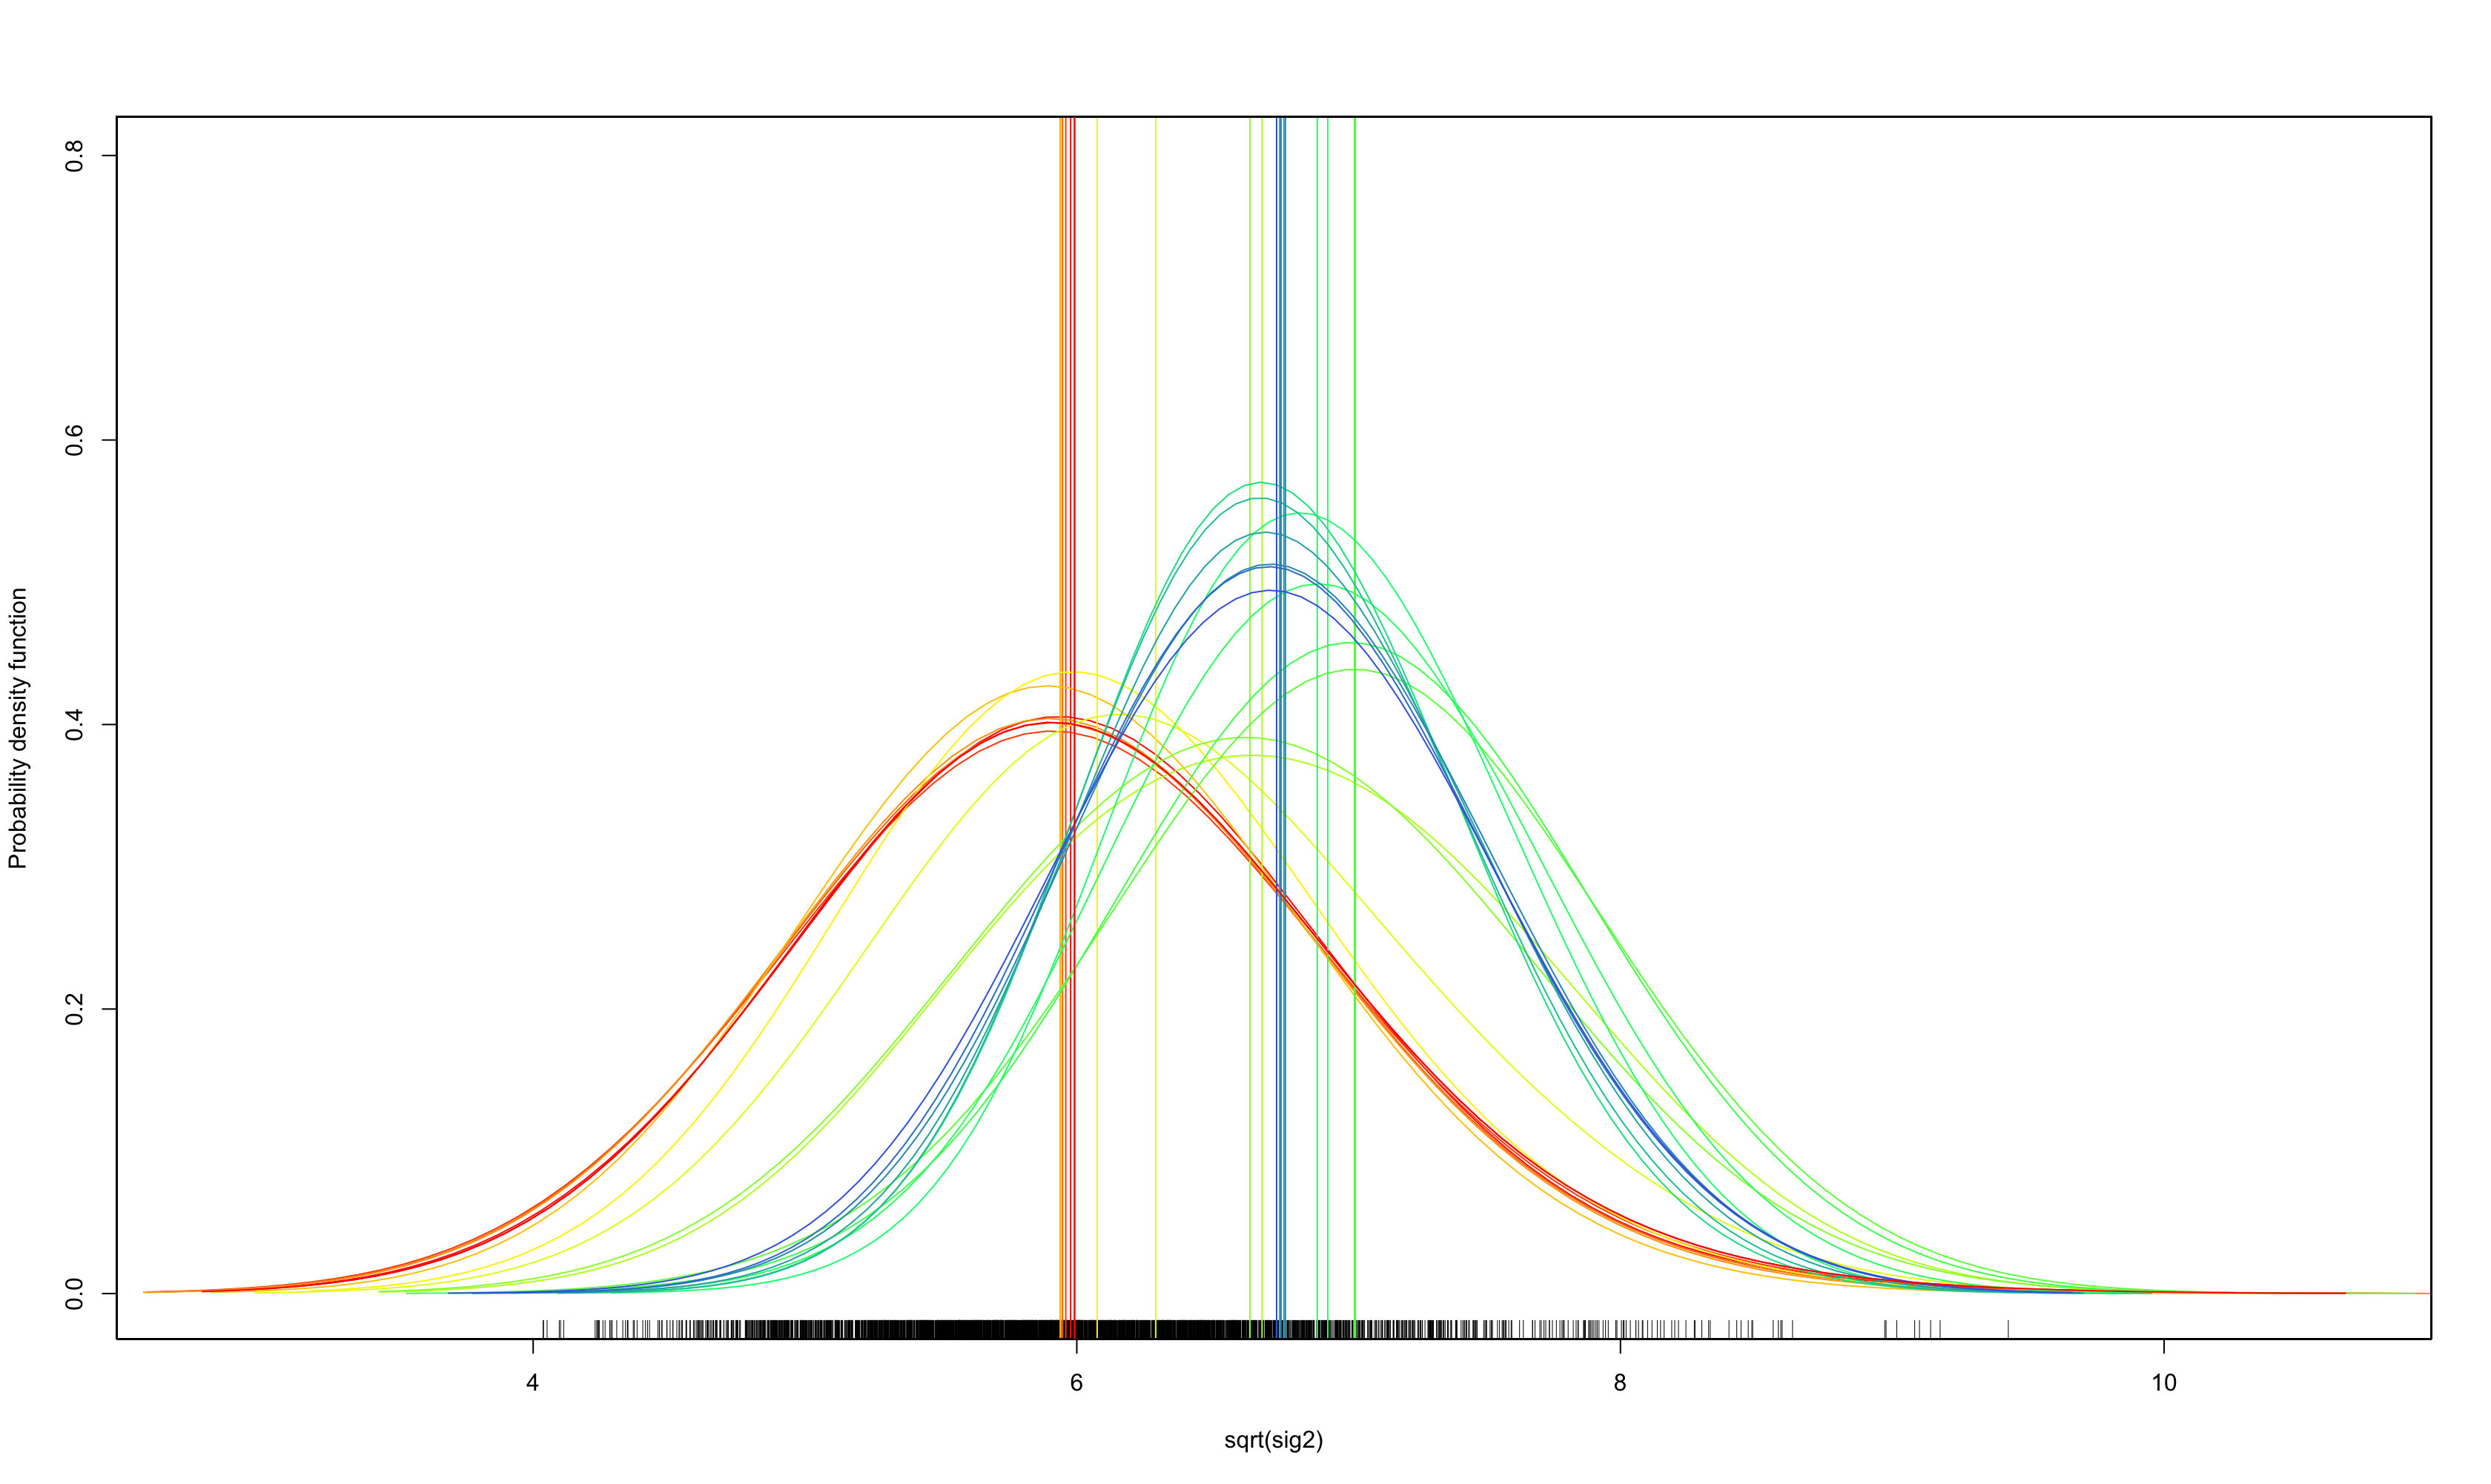
\includegraphics[width=0.8\textwidth]{ex2sigma.png}
    \vspace{0.1mm}
    \caption{Posterior means for $\sigma$ from time 2 (red) to 20 (blue); $M = 20$, $N = 3000$ (+ 1000 burn-in) qqq sizing}
    \label{sigma}
  \end{center}
\end{figure}

  \end{itemize}
  
  \item The posterior means for $y^*$ are rather lacklustre with $M = 20$ and $N = 1000$ (+ 1000 burn-in). I need to either raise $N$ to 3000 or raise $M$ above 40 to achieve better posterior means. 
  \item For some reason, $N = 4000$ and $M = 20$ performs worse in terms of posterior means of $y^*$ than $N = 3000$ and $M = 20$.
  
  \item When sampling (algorithm \ref{smcsampling}) is always included, it does not seem to matter how re-sampling is done. That is, the posterior distributions of $y^*$ do not change much.
  \item If sampling is not used, then even for large $M$ and $N$ the algorithm terminates early due to all the weights being concentrated on a single particle. I have tested up to $M = 60$ with $N = 5000$ with similar outcomes. Looking at the posterior means of $y^*$ a few time steps before the algorithm terminates, the results are poor, which suggests that sampling must be included for all except 1-dimensional problems. 

\end{itemize}

\textbf{(EX2) figures for a run with $N = 3000$ (+ 1000 burn-in), $M = 20$:}

% qqq sizing
\begin{figure}[H]
  \begin{center}
    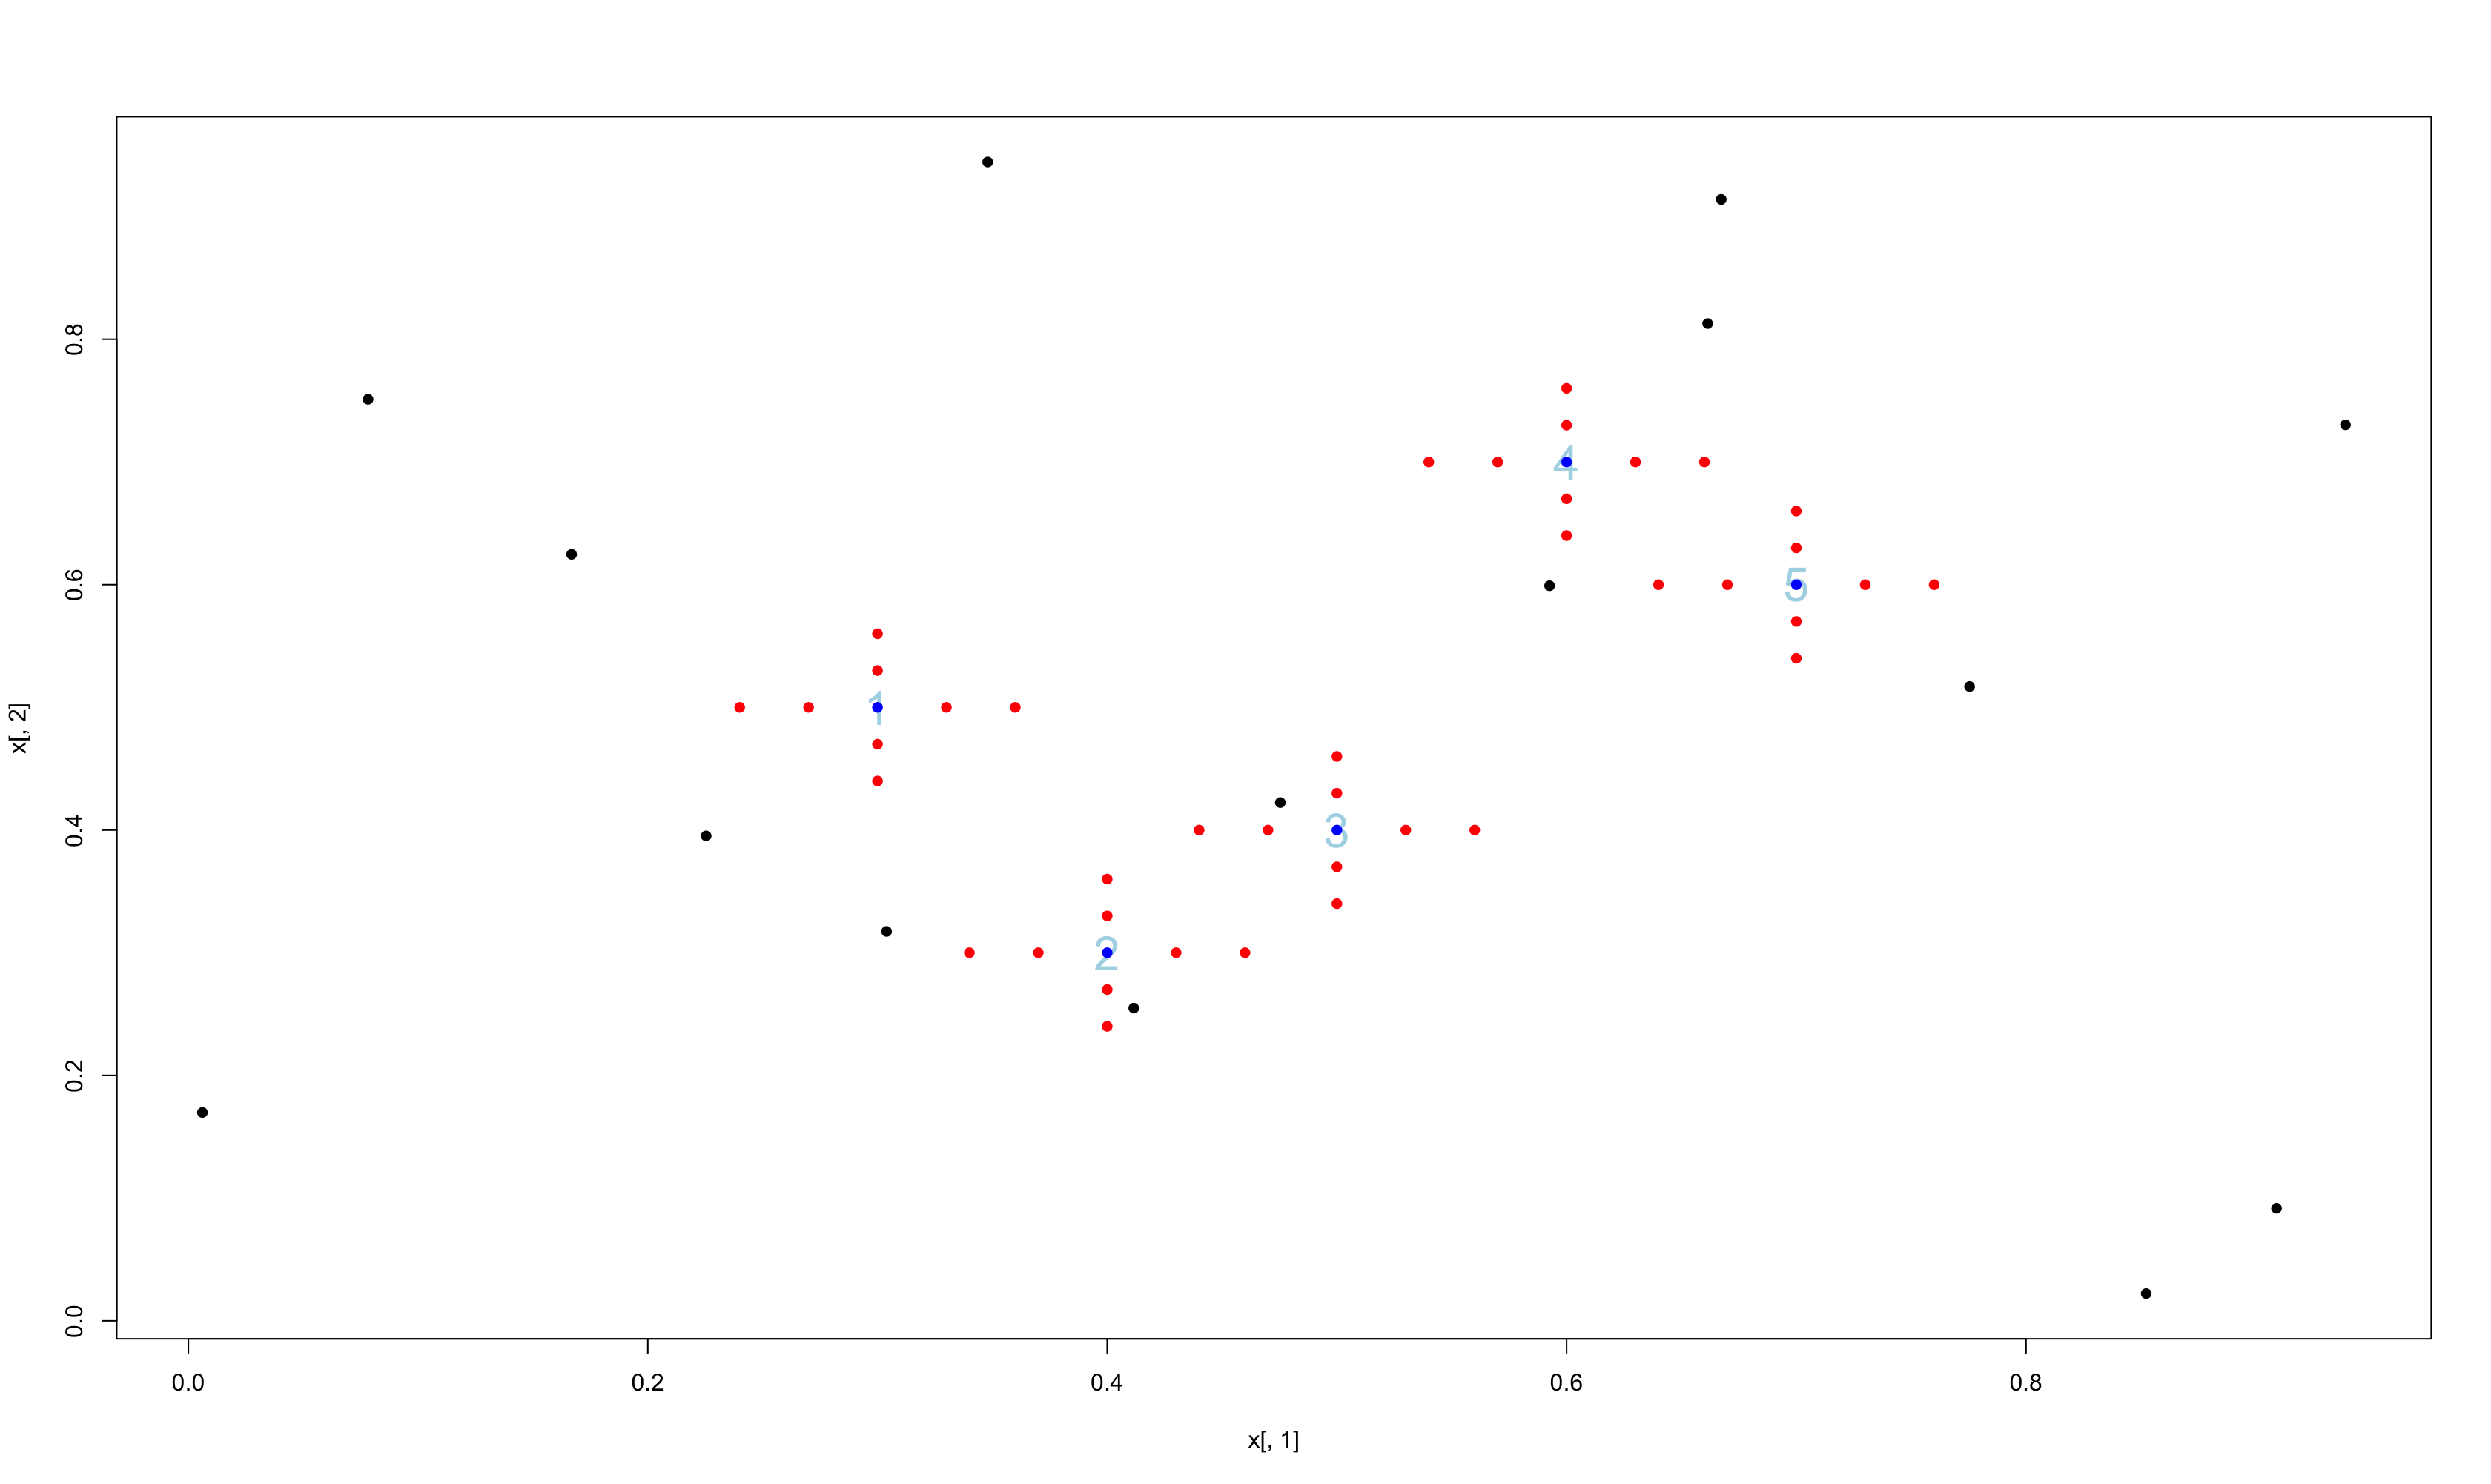
\includegraphics[width=0.98\textwidth]{ex2given.png}
    \vspace{0.1mm}
    \caption{Problem setup; black is $X$, blue is $X^*$, red is $X^\delta$.}
    \label{ex2given}
  \end{center}
\end{figure}

% qqq sizing
\begin{figure}[H]
  \begin{center}
    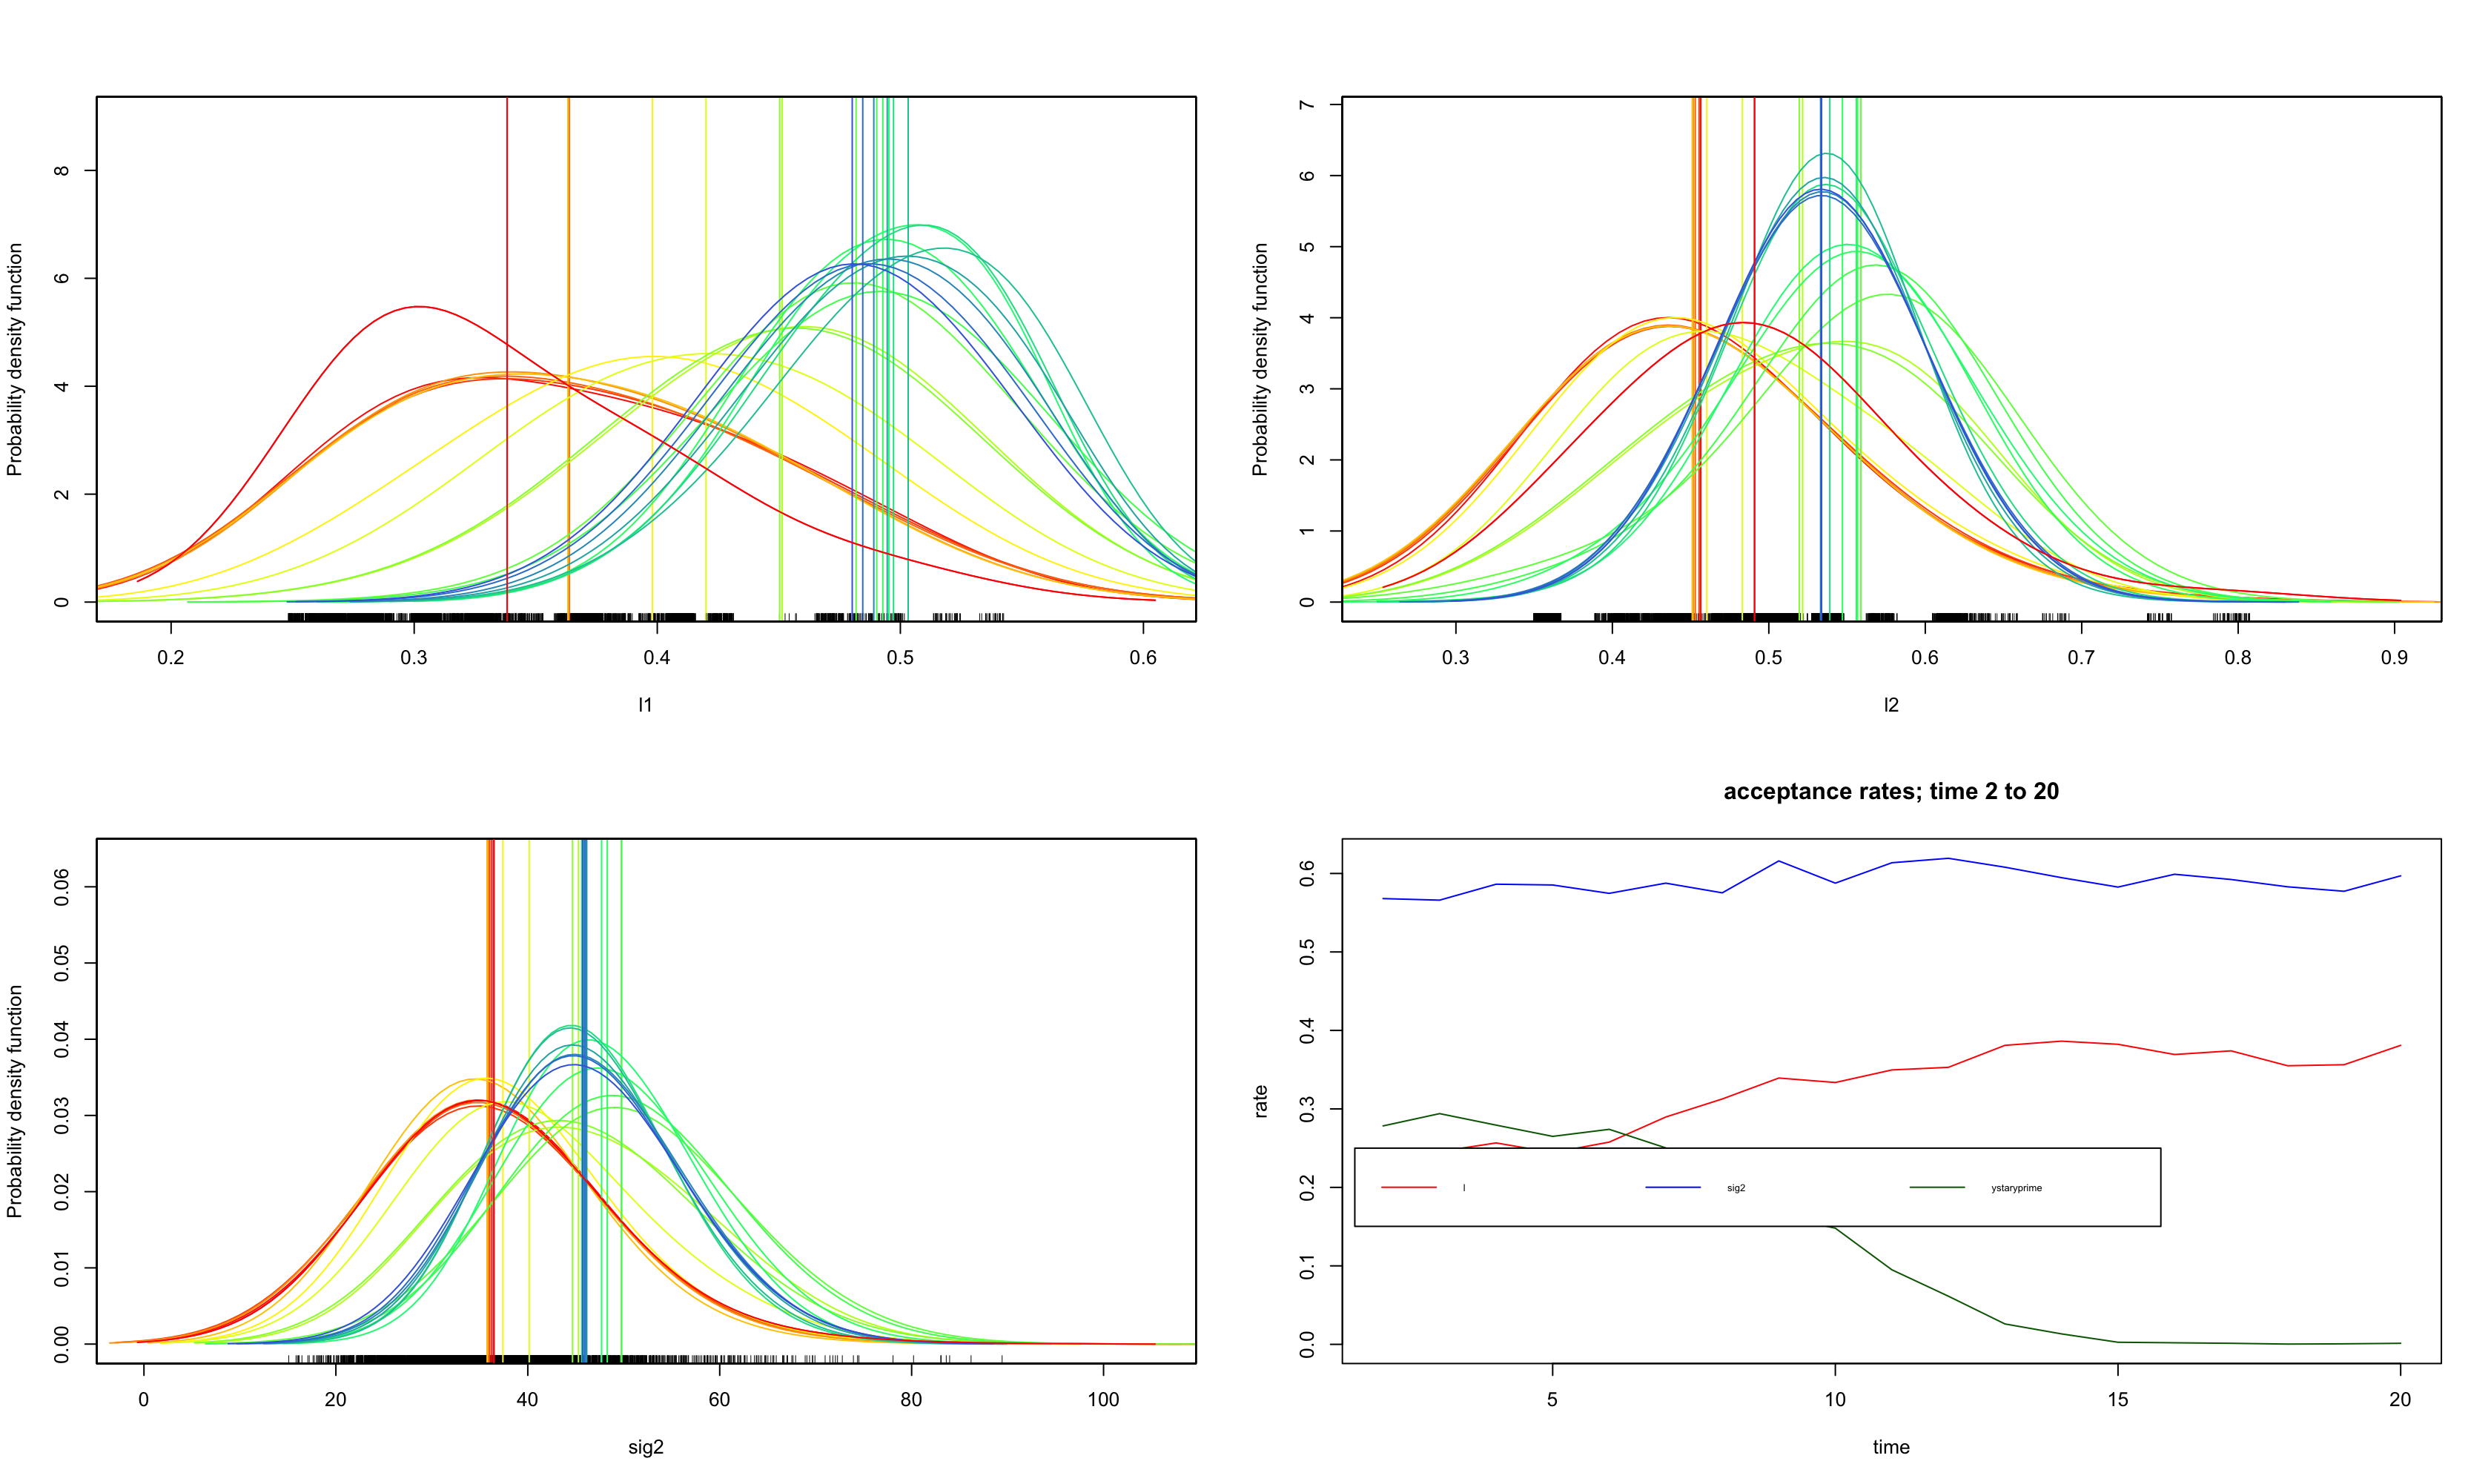
\includegraphics[width=0.98\textwidth]{ex2paras.png}
    \vspace{0.1mm}
    \caption{Posterior densities and means for $l$, $\sigma^2$ (red to blue) and acceptance rates.}
    \label{ex2paras}
  \end{center}
\end{figure}

% qqq sizing
\begin{figure}[H]
  \begin{center}
    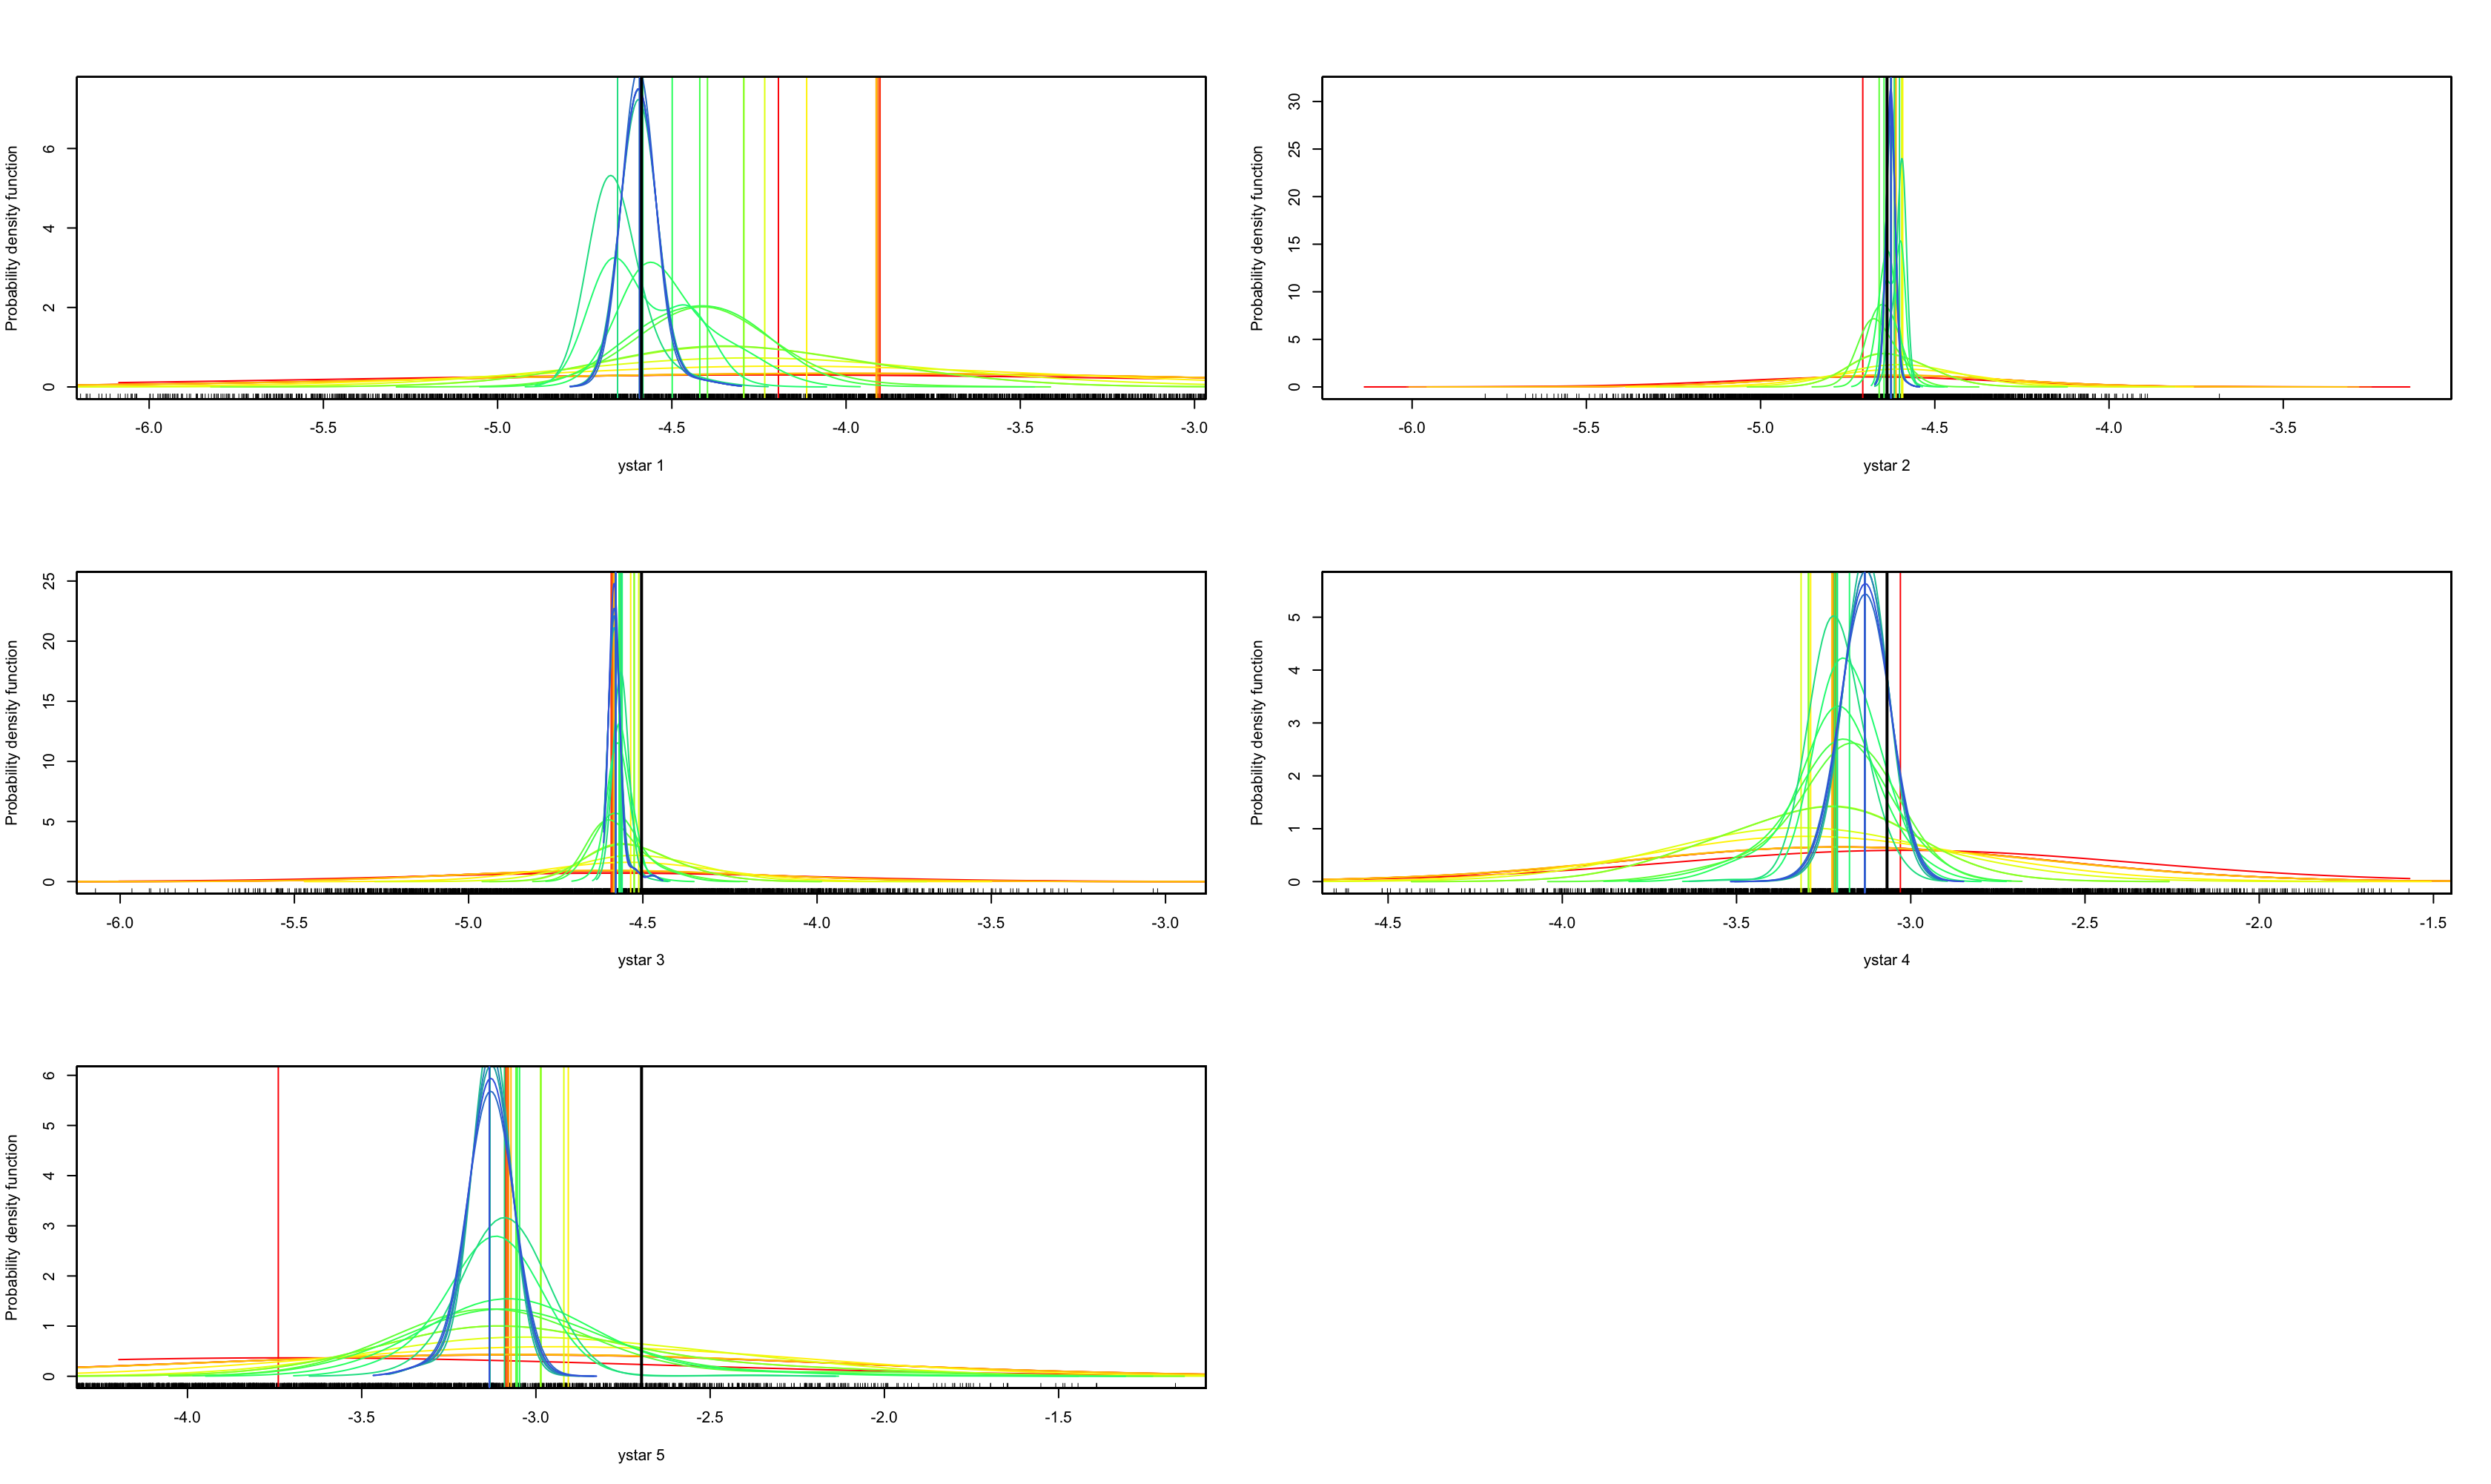
\includegraphics[width=0.98\textwidth]{ex2ystar.png}
    \vspace{0.1mm}
    \caption{Posterior densities and means for $y^*$ (red to blue).}
    \label{ex2ystar}
  \end{center}
\end{figure}


%%%%%%%%%%%%%%%%%%%%%%%%%%%%%%%%%%%%%%%%%%%%%%%%%%%%%%%%%%%%%%
\subsection{Comparing the covariance functions}
%%%%%%%%%%%%%%%%%%%%%%%%%%%%%%%%%%%%%%%%%%%%%%%%%%%%%%%%%%%%%%

\textbf{Matern}
\begin{itemize}
\item No nugget required for any examples tried so far (EX1, EX2).
\end{itemize}

\textbf{Squared exponential}
\begin{itemize}
\item A nugget is required for EX2 (I used 10e-6) everywhere a covariance matrix needs to be calculated. 
\item Seems to require many more time steps to reach a good estimate (posterior mean) for $y^*$. That is, under the same settings as when I use the Matern, the posterior means for $y^*$ appear much worse.  
\item I did not test whether a nugget is required for 1-dimensional problems
\end{itemize}

%%%%%%%%%%%%%%%%%%%%%%%%%%%%%%%%%%%%%%%%%%%%%%%%%%%%%%%%%%%%%%
%%%%%%%%%%%%%%%%%%%%%%%%%%%%%%%%%%%%%%%%%%%%%%%%%%%%%%%%%%%%%%

\section{Questions}

\begin{itemize}
\item Why does the second derivative of the Matern function have the same formula regardless of whether the derivative is in the first or second argument?
\item In EX2. are the proposal distributions for $l, \sigma^2$ still (truncated) normal and chi-squared respectively as in 1-dimension?
\item What's the step size for $l$ in higher dimensions? (I'm using a diagonal matrix multiplied by a constant.)
\item Is the step size for $l$ being continuously adapted? (I stop 2/3 of the way down the time steps.)
\item (EX2) Why are my posterior means for $y*$ moving in such an ugly manner compared to the paper's EX2 results? (Though the final posterior means generally look reasonable.)
\item (EX2) Why is my final posterior mean for $\sigma^2$ so large (looks squared) compared to that in the paper?
\item (EX2) Is EX2 following the paper's algorithm or is it only relying on re-weighting (no sampling)? 

\end{itemize}

%   BACK MATTER  %%%%%%%%%%%%%%%%%%%%%%%%%%%%%%%%%%%%%%%%%%%%%%%%%%%%%%%%%%%%%%
%
%   References and appendices. Appendices come after the bibliography and
%   should be in the order that they are referred to in the text.
%
%   If you include figures, etc. in an appendix, be sure to use
%
%       \caption[]{...}
%
%   to make sure they are not listed in the List of Figures.
%

\backmatter%
	\addtoToC{Bibliography}
	\bibliographystyle{plain}
	\bibliography{references}

\begin{appendices} % optional
	\chapter{Code}
\end{appendices}
\end{document}
